\chapter{Results}
\thispagestyle{fancy}
\chapter{Results}


\section{Asymmetries in $\theta_{abs}$ of Neutron Singles}
Using data acquired during this study, it is possible to construct $\theta_{abs}$ distributions of neutron singles, where $\theta_{abs}$ is defined as the angle between a neutron's reconstructed direction of travel and the direction of the incident photon beam.
Because the experimental design was motivated by measurements of correlated neutron doubles and not neutron singles, the methods required to obtain a neutron singles measurement are far less robust than for neutron doubles.
Nonetheless, neutron singles measurements from the photo-disintegration of D$_{2}$O showed fair agreement with known values, so these results are not totally without merit.

The distributions were calculated by normalizing a yield of photo-neutrons to the yield of neutrons from SF of $^{252}$Cf, which have no preferred direction.
However, these two yields were measured under very different experimental conditions.
This is different from the case of n-n opening angle measurements, which uses the same set of neutron events to generate two yields--uncorrected yield and correlated yield.
Another difference for these measurements is that there is no uncorrelated yield to use to subtract undesirable signals from noise and photons.

 Due to differences in experimental conditions that existed during measurements of photo-neutrons and measurements of neutrons from the SF of $^{252}$Cf, there is a high potential for systematic errors.
The photo-neutron data must be corrected for detector dead-time, which, due to the presence of the photon beam, was about an order of magnitude higher for photo-neutron measurements than for $^{252}$Cf measurements.
Accidental coincidences caused by noise and photons was estimated from data taken with a non-neutron producing aluminum target, which had to also be corrected for dead-time, and, scaled to account for the fact that the aluminum and photo-neutron data sets have different gamma detection rates.
The result was then subtracted from the photo-neutron data.
Neutrons from the SF of $^{252}$Cf do not have the same energy distribution as photo-neutrons, which could lead to incorrect results.

Despite all this, the $\theta_{abs}$ distribution for D$_{2}$O agrees moderately well with the previously established distribution, but the same may not necessarily be true for $^{238}$U and $^{232}$Th, which have a signal-to-noise ratio that is about 7 and 100 times less than for D$_{2}$O, respectively.

\begin{figure}
    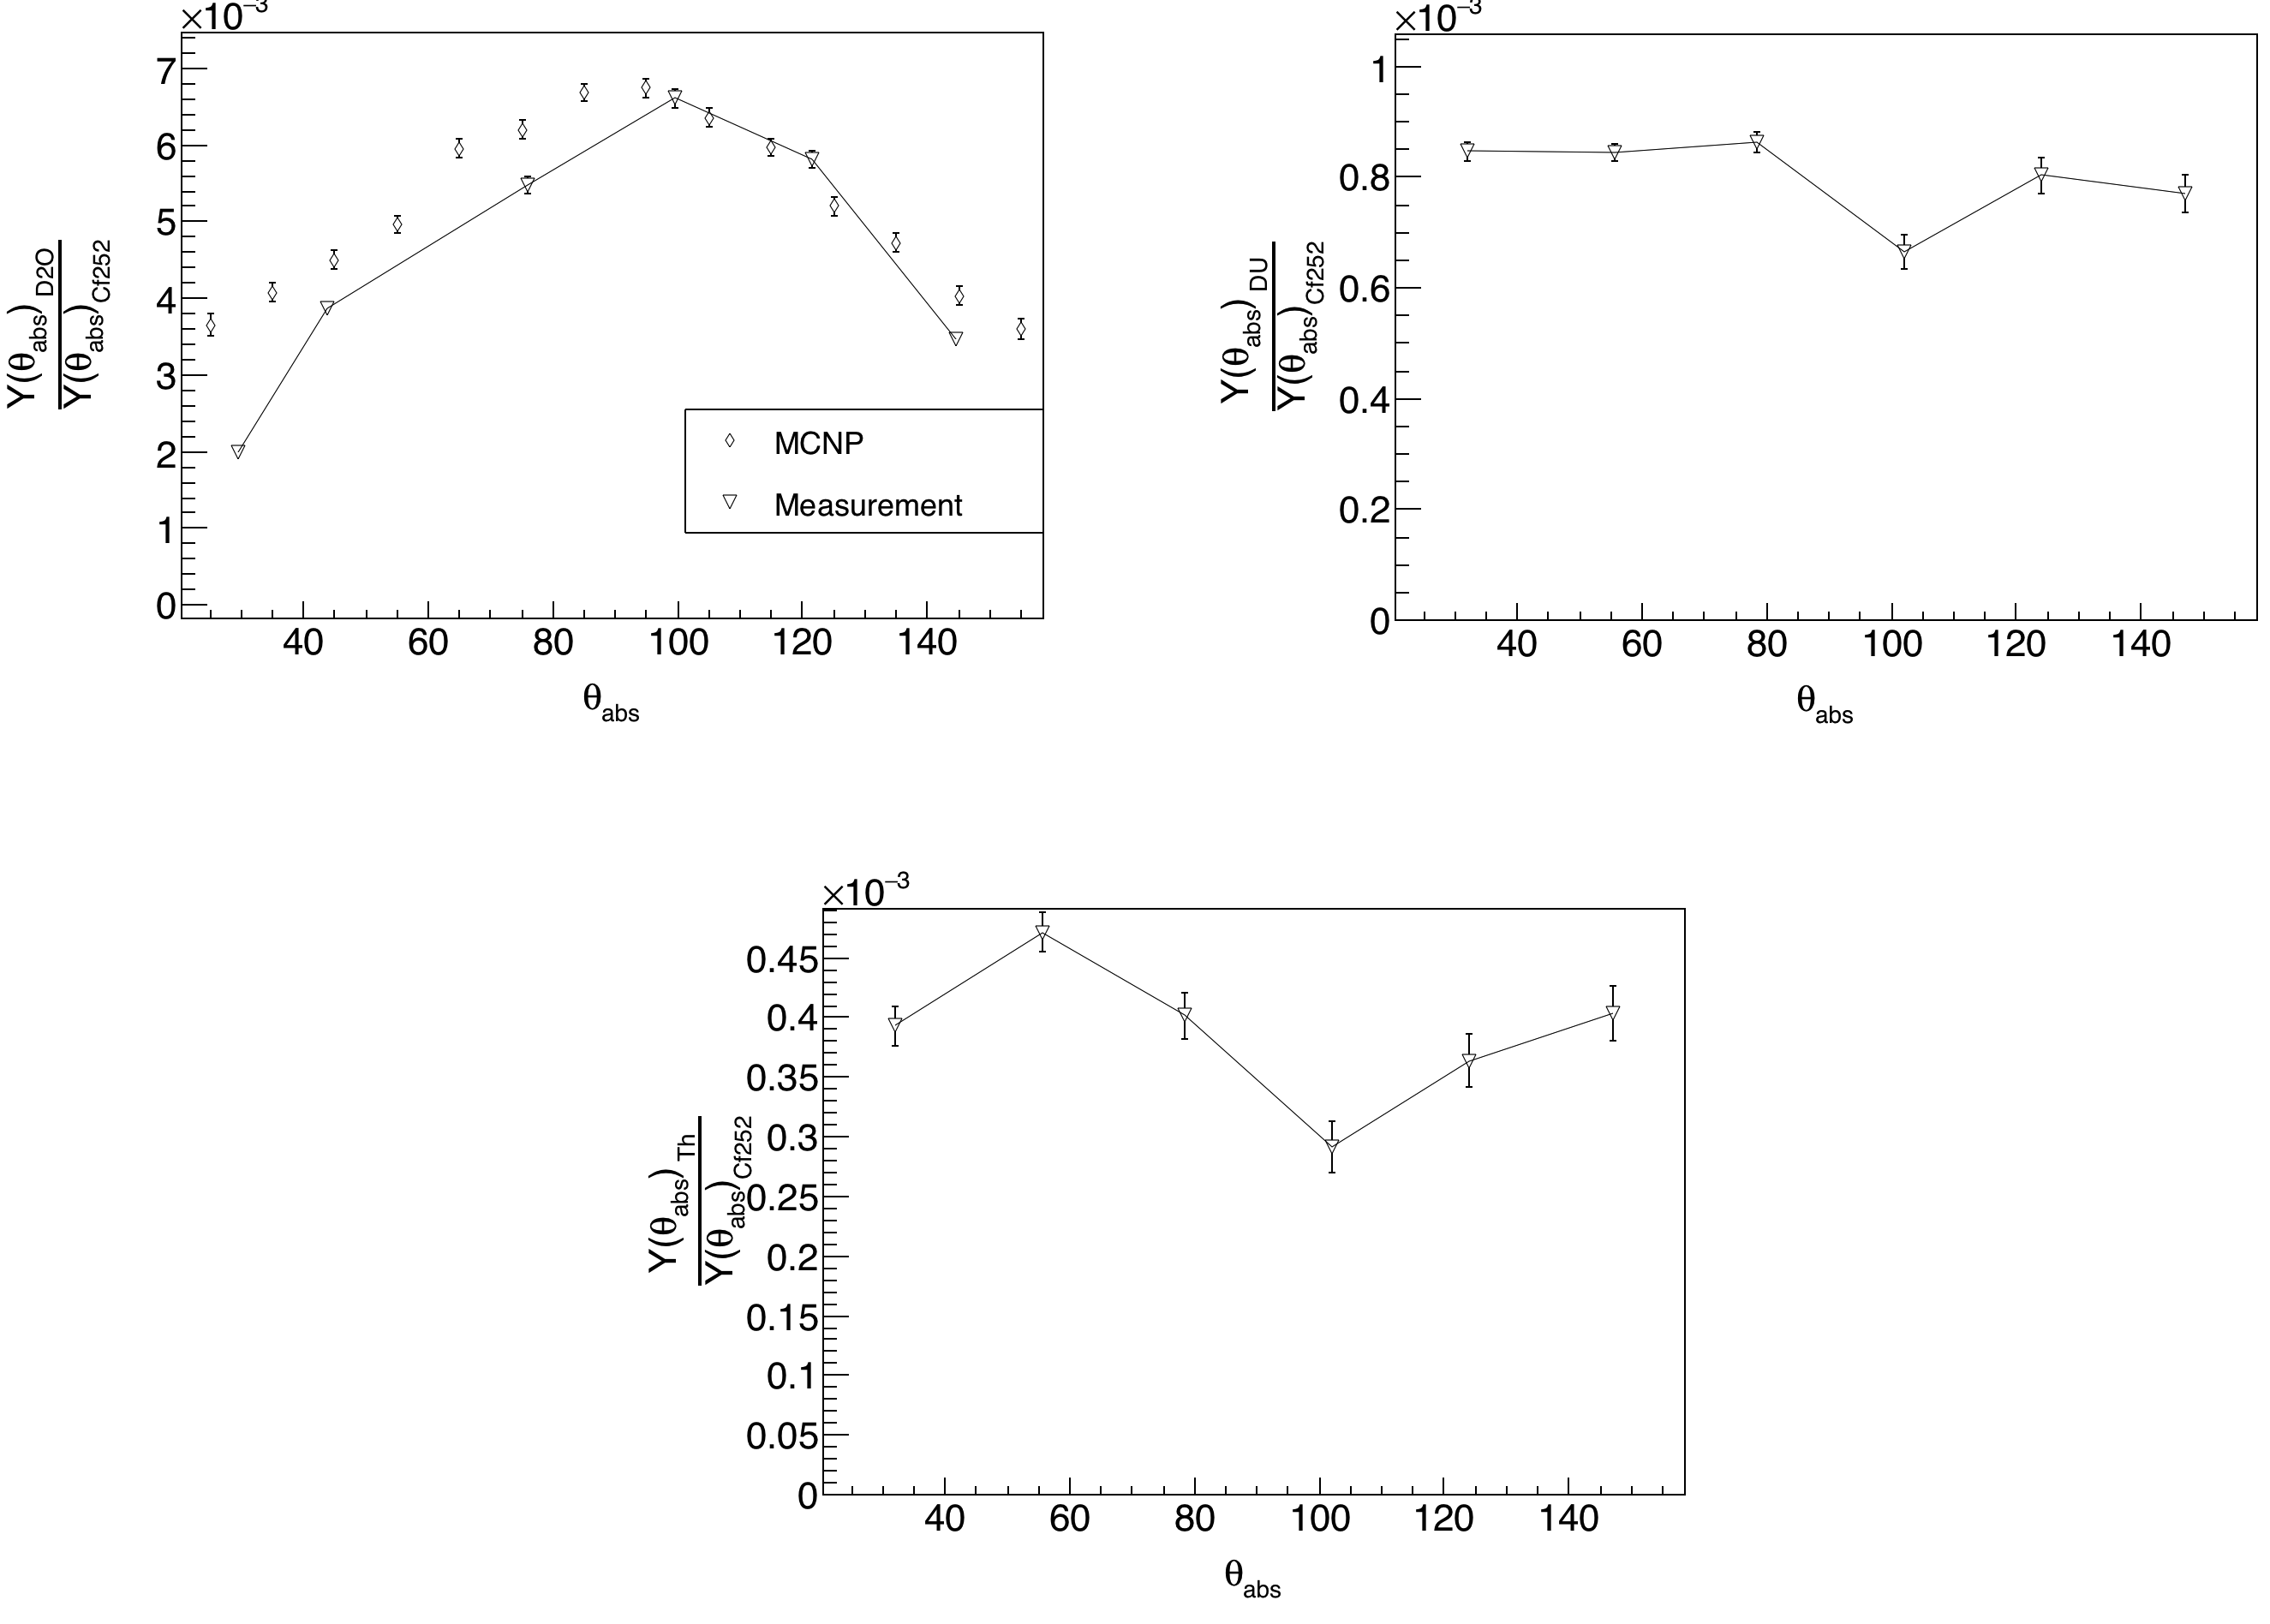
\includegraphics[width = 1\textwidth]{Content/Results/Singles.png}
    \caption{Accessory calculations were performed of the relative rates of neutrons singles as a function of $\theta_{abs}$. 
    Results are expressed as a ratio of the yield of photo-neutron singles from D$_{2}O$, $^{238}$U (DU), and $^{232}$Th, to the yield of neutron singles from the SF of $^{252}$Cf.
   The result for D$_{2}$O is in fair agreement with past measurements, however, these results have high potential for systematic errors due to the differences in experimental conditions under which the yields in the numerator and denominator (of the label for the y-axis) were measured.
       }
    \label{fig:Singles}
\end{figure}
\FloatBarrier